\newpage
\begin{center}
	\textbf{\large 2. РАЗРАБОТКА ОЦЕНОЧНОЙ ФУНКЦИИ}
\end{center}
\refstepcounter{chapter}

\addcontentsline{toc}{chapter}{2. ПРАКТИЧЕСКАЯ ЧАСТЬ}

\section{Особенности реализации kd-дерева}


В данной работе для ускорения расчетов оценочной функции была реализована структура данных kd-дерево на языке программирования C++ с поддержкой модулей. Язык программирования C++ был выбран из-за того, что библиотека для полноатомного моделирования белка и выполнения структурных изменений в белковых копмлексах, в рамках которой находится оценочная функция, реализована на языке программирования C++.

Структура данных представлеяет собой отдельный подключаемый модуль в рамках библиотеки и представляет собой C++ структуру \newline KDTree, которая хранит в себе указатель на корневой узел дерева и содержит методы:

Метод build -- принимает на вход:

\begin{itemize}
	\item массив точек, которые принадлежат дереву
	\item глубину построения дерева
	\item стартовую точку построения дерева
	\item конечную точку построения дерева
\end{itemize}

Рекурсивно строит дерево по заданному количеству точек. Возвращает указатель на построенный узел дерева

Метод search -- принимает на вход:
\begin{itemize}
	\item точку, взаимодействие с которой проверяется
	\item максимальную дистанцию радиуса взаимодействия двух точек
	\item ссылку на массив, куда будут записаны результаты
\end{itemize}

Вызывает перегруженный метод search, который дополнительными параметроми принимает узел дерева, с которым проверяется взаимодействие заданной точки, и глубину поиска. Перегруженный метод выполняет сравнение расстояния между двумя точками, если оно меньше задданой максимальной дистанции, то точка записывается в массив с результатам. Перегруженный метод рекурсивно запускает поиск для всех координат узла дерева, увеличивая глубину поиска.


\section{Особенности реализации оценочной функции}


Сначала для нахождения взаимодействующих атомов был реализован алгоритм прямого перебора всех возможных пар атомов.

Неоптимизированная функция работает следующим образом:

\begin{enumerate}
	\item берется итератор каждой цепи, загруженной в библиотеку
	\item берется итератор каждой следующей цепи, загруженной в библиотеку
	\item берется каждый атом первой цепи
	\item берется каждый атом второй цепи
	\item происходит сравнение расстояний между этими атомами и запись атомов в результат
\end{enumerate} 

Сложность алгоритма: $O(n^2 \cdot m \cdot f)$, где $n$ -- количество цепей, $m$ -- количество атомов в первой цепи, $f$ -- количество атомов во второй цепи

Позже для ускорения процесса нахождения взаимодействующих пар атомов это решение было оптимизировано. Прямой перебор всех возможных пар атомов был заменем поиском взаимодействующих атомов с использованием kd-дерева.

Оптимизированная функция работает следующим образом:

\begin{enumerate}
	\item берется итератор каждой цепи, загруженной в библиотеку, для атомов этой цепи строится kd-дерево
	\item берется итератор каждой следующей цепи, загруженной в библиотеку
	\item для каждого атома этой цепи вызывается метод search
\end{enumerate} 

Сложность алгоритма $O(n^2 \cdot m \cdot build \cdot search)$, где $n$ -- количество цепей, $m$ -- количество атомов в цепи, по которой не построено kd-дерево, $build = O(n log(n))$ -- постройка дерева, $search$ -- поиск взаимодействующих точек.

% Про данные рассказано в первой главе
%\section{Платформа и тестовые данные для численных экспериментов}
\section{Платформа для численных экспериментов}


Для проведения верификации результатов оценочной функции и просмотра результатов ускорения оценочной функции использовался удаленный сервер со следующими характеристиками: 

\begin{itemize}
	\item Операционная система -- CentOs
	\item Процессор -- Intel(R) Xeon(R) CPU E5-2650 v2 @ 2.60GHz
	\item Объем оперативной памяти -- 4.0 GB
\end{itemize}


\section{Результаты численных экспериментов}

\subsection{Поиск взаимодействующих атомов}


На рисунках \ref{1tm1}--\ref{1kxq} представлено сравнение времени поиска взаимодействующих атомов для двух белков различными инструментами. Как видно из результатов, алгоритм с применением прямого перебора всех атомов работает в разы медленее трех других алгоритмов. Алгоритмы с применением kd-дерева работают быстрее остальных алгоритмов, алгоритм с использованием оптимизированного kd-дерева работает за наименьшее среди всех функций время. Программный комплекс Rossetta работает чуть медленее алгоритмов с использованием kd-дерева.

Обозначения на рисунках \ref{1tm1}--\ref{1kxq}
\begin{itemize}
	\item nn -- алгоритм прямого перебора всех атомов
	\item Rosetta -- программный комплекс Rosetta
	\item k-d -- алгоритм с использованием Kd-дерева
	\item k-d-opt -- алгоритм с использованием оптимизированного Kd-дерева
\end{itemize}

\begin{figure}[h!]
	\centering
	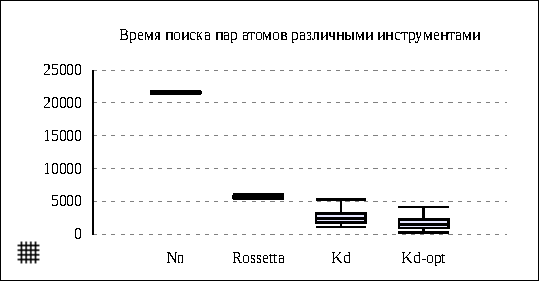
\includegraphics[width=1.0\linewidth]{images/plotsvg.pdf}
	\caption{Время поиска пар атомов для белка 1TM1 различными инструментами}
	\label{1tm1}
\end{figure}

\begin{figure}[h!]
	\centering
	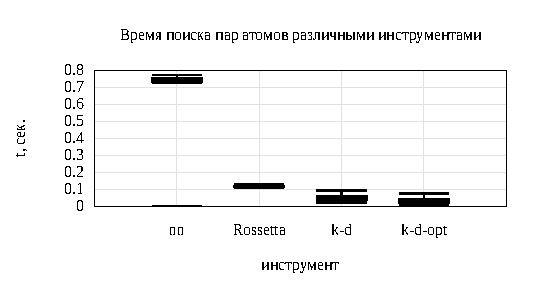
\includegraphics[width=1.0\linewidth]{images/plotsvg1.pdf}
	\caption{Время поиска пар атомов для белка 1KXQ различными инструментами}
	\label{1kxq}
\end{figure}


\subsection{Верификация выполняемых оценок}


На рисунках~\ref{first}--\ref{second} приведены результаты численных оценок для 84 комплексов. Средствами пакета CHARMM выполнена оценка энергии для представленных в разработанной оценочной функции компонент. Для полученных значений рассчитан линейный коэффициент корреляции Пирсона.

Следует отметить, что представленная на рисунках оценка включает в~себя внутримолекулярные взаимодействия. Для этого в~оценочной функции и~в пакете CHARMM использовалась так называемая схема~1-3, где при формировании списка взаимодействующих пар атомов исключаются пары, которые связаны ковалентно~(схема~1-2), а~также пары, <<соединенные>> одним общим атомом. При рассмотрении компонент комплекса в~виде <<твёрдых>> тел внутримолекулярные взаимодействия изменяться не будут, поэтому при моделировании процесса образования комплекса достаточно выполнить их оценку только один раз и~затем рассматривать взаимодействия только между атомами компонент комплекса.

\begin{figure}[h!]
	\centering
	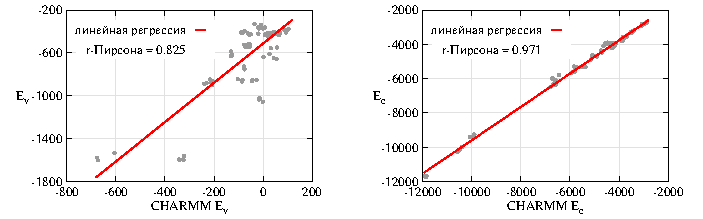
\includegraphics[width=1.0\linewidth]{images/first.pdf}
	\caption{Результаты численного эксперимента для потенциала Леннард-Джонса и для потенциала Кулона}
	\label{first}
\end{figure}

\begin{figure}[h!]
	\centering
	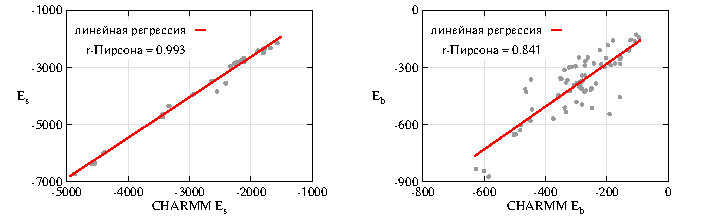
\includegraphics[width=1.0\linewidth]{images/second.pdf}
	\caption{Результаты численного эксперимента для неявного растворителя и для оценки энергии связывания}
	\label{second}
\end{figure}

В простейшем случае процесс связывания описывается моделью вида ключ-замок, которая представляется в~виде $A+B\leftrightarrow AB$, где $A$ и~$B$ являются компонентами комплекса. С~помощью разработанной целевой функции возможно оценить энергию этого взаимодействия. На рисунке~\ref{second} продемонстрирована оценка энергии связывания без учета растворителя, которая определяется по следующей формуле:
\begin{equation}
	E_{b}=\left[E_{v}^{AB} + E_{c}^{AB}\right] - \left[E_{v}^{A} + E_{c}^{A} + E_{v}^{B} + E_{c}^{B}\right].
	\label{bind}
\end{equation}

В численном эксперименте в начальном PDB файле представлен образованный комплекс $AB$. При определении энергии связывания \eqref{bind} вычисляется разница между оценкой энергии комплекса в связанном состоянии и оценками энергий в свободном состоянии для каждого компонента в отдельности. В данном случае оценка энергии растворителя исключена для сравнения результатов оценки взаимодействия только на основе двух слагаемых оценочной функции.

На рисунке \ref{third} показано сравнение оценок энергии связывания, вычисленные с помощью нашей функции -- обозначение $F_s$ на графике -- и инструментами CHARMM и Rosetta. Для наглядности посчитана линейная регрессия и коэффициент корреляции Пирсона.

\begin{figure}[h!]
	\centering
	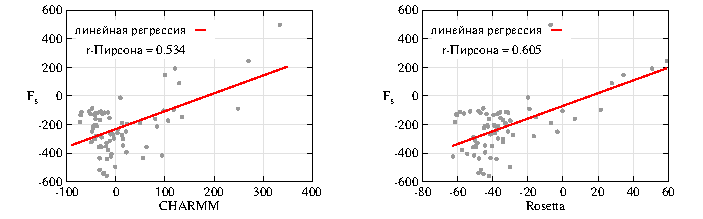
\includegraphics[width=1.0\linewidth]{images/third.pdf}
	\caption{Сравнение оценок энергии связывания, вычисленные с помощью различных интсрументов}
	\label{third}
\end{figure}
